\documentclass[11pt]{article}
\usepackage{amsmath}
\usepackage{booktabs}
\usepackage[margin=1in]{geometry}
\usepackage{graphicx}
\usepackage[final]{microtype}
\usepackage{xcolor}
\PassOptionsToPackage{hyphens}{url}
\usepackage{hyperref}
\usepackage{longtable}
\usepackage{tikz}
\usetikzlibrary{arrows.meta,positioning}

\definecolor{templateInk}{HTML}{172033}
\definecolor{templateAccent}{HTML}{0B5C6B}
\definecolor{templateMuted}{HTML}{4D5B68}
\definecolor{templateSoft}{HTML}{EEF6F7}

\hypersetup{
  colorlinks=true,
  linkcolor=templateAccent,
  citecolor=templateAccent,
  urlcolor=templateAccent,
  pdftitle={Reusable arXiv Article Template},
  pdfauthor={Author Name},
  pdfsubject={arXiv manuscript template},
  pdfkeywords={arXiv, LaTeX, manuscript, reproducibility}
}

\urlstyle{same}
\emergencystretch=2.5em
\clubpenalty=10000
\widowpenalty=10000
\displaywidowpenalty=10000
\setlength{\parskip}{0.28em plus 0.06em minus 0.03em}
\setlength{\parindent}{1.15em}
\renewcommand{\arraystretch}{1.12}
\setlength{\tabcolsep}{5pt}

\makeatletter
\renewcommand\section{\@startsection{section}{1}{\z@}%
  {-2.2ex plus -0.6ex minus -0.2ex}%
  {1.0ex plus 0.2ex}%
  {\normalfont\Large\bfseries\color{templateInk}}}
\renewcommand\subsection{\@startsection{subsection}{2}{\z@}%
  {-1.6ex plus -0.4ex minus -0.2ex}%
  {0.55ex plus 0.15ex}%
  {\normalfont\large\bfseries\color{templateInk}}}

\renewcommand{\maketitle}{%
  \begin{center}
    {\LARGE\bfseries\color{templateInk}\@title\par}
    \vspace{0.8em}
    {\large\color{templateMuted}\@author\par}
    \vspace{0.45em}
    {\color{templateMuted}\@date\par}
    \vspace{0.8em}
    {\color{templateAccent}\rule{0.72\linewidth}{0.8pt}\par}
  \end{center}
  \vspace{0.8em}
}
\makeatother

\renewenvironment{abstract}
  {\begin{center}\begin{minipage}{0.92\linewidth}\small\noindent\textbf{\color{templateInk}Abstract.}\ }
  {\end{minipage}\end{center}\vspace{0.7em}}

\newcommand{\glslink}[2]{\hyperlink{gloss:#1}{#2}}
\newcommand{\abblink}[2]{\hyperlink{abbr:#1}{#2}}

\title{Reusable arXiv Article Template: A clean manuscript and packaging workflow}
\author{Author Name\\
Department or Institute\\
University or Organisation}
\date{\today}

\begin{document}

\maketitle

\begin{abstract}
This template provides a compact arXiv-ready article layout with source-package checks, citation reconciliation, privacy auditing, and deterministic upload packaging. The style is intentionally plain: it uses standard LaTeX packages, restrained colour, readable typography, source-safe TikZ figures, and explicit declarations. Replace this abstract with a concise statement of the problem, method, evidence, and contribution. Keep claims tied to evidence and avoid implying external submission, review, or acceptance until those events have occurred.
\end{abstract}

\section*{Plain-language summary}
Use this optional section when the manuscript benefits from a short explanation for adjacent-field readers. State the problem in ordinary language, describe what the paper contributes, and explain what the paper does not claim.

\section{Introduction}
Introduce the problem, why it matters, and the gap this manuscript addresses. Cite foundational or standards references only when they directly support the claim being made \cite{lamport-1994,w3c-rdf11-concepts}. Keep the final paragraph of the introduction focused on the contribution.

The contribution is threefold. First, the manuscript states a concrete research or resource problem. Second, it explains the method or design surface used to address that problem. Third, it packages the evidence, limitations, data/code availability, and submission checks so that readers can inspect the path from source material to claim.

\section{Results}
\subsection{A compact evidence surface}
Summarise the main findings or artefacts. Table~\ref{tab:evidence-surfaces} shows a reusable way to separate evidence types from claims.

\begin{table}[ht]
\centering
\caption{Evidence surfaces used to support manuscript claims.}
\label{tab:evidence-surfaces}
\begin{tabular}{p{0.32\linewidth}p{0.56\linewidth}}
\toprule
Surface & Role in the claim set \\
\midrule
Primary artefact & The main data, model, software, resource, or theoretical object. \\
Validation checks & Executable tests, reproducibility checks, or independent consistency checks. \\
Comparison package & Source inventory, related work, baselines, or mapped concepts. \\
Submission package & Clean source bundle, privacy audit, PDF build, and checksums. \\
\bottomrule
\end{tabular}
\end{table}

\subsection{A reusable visual style}
Figure~\ref{fig:workflow} demonstrates the built-in TikZ style. Prefer source figures or arXiv-safe PDF/PNG/JPG assets.

\begin{figure}[ht]
\centering
\resizebox{\linewidth}{!}{%
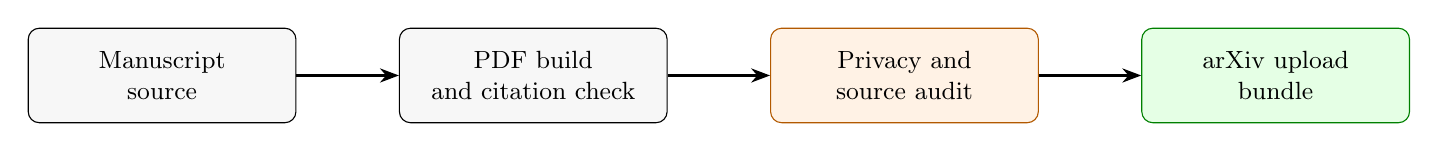
\begin{tikzpicture}[
  node distance=10mm and 13mm,
  box/.style={draw, rounded corners, align=center, minimum width=34mm, minimum height=12mm, font=\small, fill=gray!6},
  done/.style={box, fill=green!10, draw=green!50!black},
  review/.style={box, fill=orange!10, draw=orange!70!black},
  arrow/.style={-{Stealth[length=2.4mm]}, thick}
]
\node[box] (draft) {Manuscript\\source};
\node[box, right=of draft] (build) {PDF build\\and citation check};
\node[review, right=of build] (audit) {Privacy and\\source audit};
\node[done, right=of audit] (bundle) {arXiv upload\\bundle};
\draw[arrow] (draft) -- (build);
\draw[arrow] (build) -- (audit);
\draw[arrow] (audit) -- (bundle);
\end{tikzpicture}}
\caption{Reusable arXiv source workflow. The same sequence can run locally and in GitHub Actions.}
\label{fig:workflow}
\end{figure}

\section{Methods}
\subsection{Manuscript build}
The local manuscript build compiles `paper/paper.tex` with a detected TeX engine. The preferred path is Tectonic when available because it is portable in local Codex environments; GitHub Actions can use a TeX Live setup with `latexmk` or `pdflatex` when stricter arXiv parity is required.

\subsection{Citation reconciliation}
Citation keys in the LaTeX source are checked against `paper/references.csl.json` and the explicit `\verb|\bibitem|` list. This is deliberately simple. It catches missing or orphaned keys without forcing a particular bibliography manager.

\subsection{Source-package checks}
The arXiv preflight builds a source directory, removes auxiliary files, checks filenames, audits for local paths and credential-like strings, and writes an upload-ready tarball with a JSON manifest and SHA-256 checksums.

\section{Limitations}
This template does not prove that a manuscript is scientifically correct, externally reviewed, or accepted by arXiv. It only packages source hygiene, formatting, citation reconciliation, and reproducibility checks. Human review, arXiv upload, rendered-PDF inspection, and identifier recording remain external steps.

\section{Data and code availability}
Replace this paragraph with repository, data, software, or archive links. For local validation, run:
\begin{itemize}
\item \texttt{make manuscript-pdf}
\item \texttt{make arxiv-upload-ready}
\item \texttt{make test}
\end{itemize}

\section{Declarations}
\textbf{Ethics approval and consent to participate.} Not applicable unless the manuscript reports human participant, animal, clinical, or other regulated data.

\textbf{Competing interests.} The author declares no competing interests, or states them here.

\textbf{Funding.} State funding sources or say that no specific funding was received.

\textbf{Author contributions.} State contribution roles here.

\textbf{Acknowledgements.} State acknowledgements here.

\textbf{AI and tool use.} State any AI-assisted drafting, coding, review, or source-checking tools used, and keep final responsibility with the human author.

\appendix
\setcounter{figure}{0}
\renewcommand{\thefigure}{A\arabic{figure}}
\renewcommand{\theHfigure}{appendix.A\arabic{figure}}
\section{Supplementary Notes}
Use appendices for visual summaries, extra checks, or submission-package notes that are useful for reviewers but too detailed for the main text.

\begin{thebibliography}{99}

\bibitem{lamport-1994}
Leslie Lamport.
\newblock \emph{LaTeX: A Document Preparation System}.
\newblock Addison-Wesley, 1994.

\bibitem{w3c-rdf11-concepts}
W3C RDF Working Group.
\newblock \emph{RDF 1.1 Concepts and Abstract Syntax}.
\newblock 2014. \url{https://www.w3.org/TR/rdf11-concepts/}.

\end{thebibliography}

\clearpage
\section*{Glossary}
\addcontentsline{toc}{section}{Glossary}
\begin{description}
\item[\hypertarget{gloss:source-package}{Source package}] A cleaned set of source files suitable for upload to arXiv.
\item[\hypertarget{gloss:privacy-audit}{Privacy audit}] A scan for local paths, hidden files, and credential-like text before packaging.
\end{description}

\clearpage
\section*{Abbreviations}
\addcontentsline{toc}{section}{Abbreviations}
\begin{description}
\item[\hypertarget{abbr:csl}{CSL}] Citation Style Language.
\item[\hypertarget{abbr:pdf}{PDF}] Portable Document Format.
\end{description}

\end{document}

